\subsection*{Solution 7}

\begin{itemize}
\item[(a)]

$q$ is continuous on $\Complex$, and its conjugate
$\overline{q}(z) = z+1+i$
is entire, hence $q$ is a model fluid flow.\hbm{D2}{1.14}

\item[(b)]

The complex potential function, $\Omega(z)$ for $q$ is a primitive of
$\overline{q}$, so
\[
\Omega(z) = \frac{z^2}{2}+(1+i)z
\]
Now, for $z=x+iy$
\begin{eqnarray*}
\Omega(x+iy)
	&=& \frac{ (x+iy)^2 }{ 2 } + (1+i)(x+iy) \\
	&=& \frac{ x^2-y^2 +2xyi }{2} + x + iy + ix - y \\
	&=& x^2/2 - y^2/2 + x - y + i(x + y + xy) \\
	&=& \Phi(x,y) + i\Psi(x,y)
\end{eqnarray*}
So, $q$ has streamline $\Psi(x,y)=x+y+xy=C$, for constant $C$.\hbm{D2}{2.1}

For the streamline through the point 1, $\Psi(1,0) = 1$, so, the
streamline through point 1 has the equation $x+y+xy=1$, a hyperbola.


%
%	Sketches for Q7
%

%
%	Plot of the streamline
%
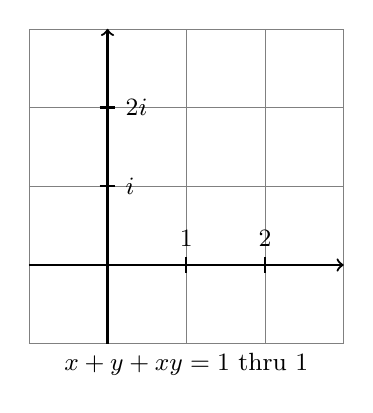
\begin{tikzpicture}
	% grid for draft only
	\draw [help lines] (-1,-1) grid (3,3);
	% legend
	\draw (1,-1) node[below] {\small $x+y+xy=1$ thru 1};
	% the X-axis
	\draw[->,thick] (-1,0)--(3,0);
	\draw[thick] (1,-0.1) -- (1,0.1) node[above=0pt] {\small $1$};
	\draw[thick] (2,-0.1) -- (2,0.1) node[above=0pt] {\small $2$};
	% the Y-axis
	\draw[->,thick] (0,-1)--(0,3);
	\draw[thick] (-0.1,1) -- (0.1,1) node[right=0pt] {\small $i$};
	\draw[thick] (-0.1,2) -- (0.1,2) node[right=0pt] {\small $2i$};
	% the hyperbola
	\draw[thick,domain=-0.5:3] plot function{(1-x)/(1+x)};
\end{tikzpicture}


Since $q(1)=2-i$, the direction of the flow is from top-left to
bottom-right.

\item[(c)]
Using the results from part (a) and part (b):\hbm{D2}{1.10}\hbm{B1}{2.1}
\begin{eqnarray*}
C_\Gamma
	&=& \RE \int_\Gamma \overline{q}(z)\,dz \\
	&=& \RE \int_\Gamma (z+1+i)\,dz \\
	&=& \RE \int_0^4 (\gamma(t)+1+i)\gamma'(t)\,dt \\
	&=& \RE \int_0^4 (t+1+i)\,dt \\
	&=& \RE \left[ t^2/2+(1+i)t \right]_0^4 \\
	&=& \RE ( 16/2 +4+4i ) \\
	&=& 12
\end{eqnarray*}

\end{itemize}

